\documentclass[11pt]{cernrep}
\usepackage{graphicx,epsfig}
\bibliographystyle{lesHouches}

\usepackage{cite}
\usepackage{amsmath}
\usepackage[colorlinks=True,citecolor=blue]{hyperref}

\newcommand{\GeV}{\,\mathrm{GeV}}
\newcommand{\TeV}{\,\mathrm{TeV}}
\newcommand{\ie}{i.e.\ }
\newcommand{\eg}{e.g.\ }
\newcommand{\order}[1]{{\cal O}\left(#1\right)}
\newcommand{\avg}[1]{\left\langle\smash{#1}\right\rangle}
\newcommand{\as}{\alpha_s}
\newcommand{\ycut}{y_{\text{cut}}}
\newcommand{\zcut}{z_{\text{cut}}}
\newcommand{\fcut}{f_{\text{cut}}}
\newcommand{\ftrim}{f_{\text{trim}}}
\newcommand{\Rtrim}{R_{\text{trim}}}
\newcommand{\rtrim}{r_{\text{trim}}}
\newcommand{\zprune}{z_{\text{prune}}}
\newcommand{\Rprune}{R_{\text{prune}}}
\newcommand{\rprune}{r_{\text{prune}}}
\newcommand{\e}{\varepsilon}
\newcommand{\cf}{C_{F}}
\newcommand{\ca}{C_{A}}
\newcommand{\nf}{n_{F}}
\newcommand{\MSb}{\overline{\rm MS}}
\newcommand{\W}{{\rm W}}
\newcommand{\TiTj}{{\bf T}_i \cdot {\bf T}_j}
\newcommand{\ord}{\mathcal{O}}
\newcommand{\gstrong}{g_s}
\newcommand{\muNP}{\mu_\text{NP}}
\newcommand{\amax}{a_2}
\newcommand{\amin}{a_1}
\newcommand{\tlambda}{\tilde{\lambda}}



\renewcommand{\d}{\mathrm{d}}

\newcommand{\SD}{SoftDrop\xspace}
\newcommand{\ttt}[1]{{\small\texttt{#1}}}
\newcommand{\fastjet}{\texttt{FastJet}\xspace}
\newcommand{\fjcontrib}{\texttt{fjcontribtJet}\xspace}

\usepackage{color}
\definecolor{darkgreen}{rgb}{0,0.5,0}
\definecolor{darkblue}{rgb}{0,0,0.7}
\definecolor{darkred}{rgb}{0.5,0,0.0}

\newcommand{\sm}[1]{\textbf{\color{darkgreen}  [#1 -- sm]}}


\begin{document}

\section{Jet Studies: Four decades of gluons\protect\footnote{Section coordinators: S.~Marzani and B.~Nachman}$^{,}$~\protect\footnote{Contributing authors: S.~Amoroso, P.~Azzurri, H.~Brooks, S.~Forte, P.~Gras, Y.~Haddad, J.~Huston, A.~Larkoski, M.~Le Blanc, P.~Loch, K.~Long, E.~Metodiev, D.~Napoletano, S.~Prestel, P.~Richardson, F.~Ringer, J.~Roloff, D.~Soper, G.~Soyez, V.~Theeuwes}}

Studies related to gluon jets have played a key role in particle and nuclear physics since their discovery at PETRA exactly \textbf{four decades} prior to the 2019 Les Houches workshop.  This section investigates gluon fragmentation at the LHC, covering nearly \textbf{four decades} in energy scales.  Low energy scales involving gluon (sub)jets are studied from the point of view of hadronization and Monte Carlo tuning.  Higher-order effects in parton shower programs are investigated using deep learning.  Gluon jet rejection is considered in the context of vector boson fusion/scattering processes.  One of the main studies at this Les Houches was a study about the usefulness of a gluon jet differential cross section measurement in the context of parton distribution functions.  Gluon jet identification was also briefly discussed for searches at the highest energies accessible at the LHC.

\subsection{Introduction}
\label{sec:jets:intro}

Jets are collimated sprays of hadrons that emerge from high energy quarks and gluons and are an important asset or significant nuisance in a a majority of collider particle physics analyses.  Understanding jets and their internal structure (jet substructure~\cite{Abdesselam:2010pt,Altheimer:2012mn,Altheimer:2013yza,Adams:2015hiv,Asquith:2018igt,Larkoski:2017jix}) will directly or indirectly address a variety of fundamental questions in particle and nuclear physics.  One of the first studies related to jet substructure occurred nearly four decades ago, with the direct discovery of the gluon at PETRA~\cite{Brandelik:1979bd,Barber:1979yr,Berger:1979cj,Bartel:1979ut,Ellis:2014rma}.  It was of paramount importance at the time to study differences between jets initiated by quarks (quark jets) and jets initiated by gluons (gluon jets) in order to categorize the properties of the new boson.  This complex topic is still an active area of research in the present day and was the subject of the 2015 Les Houches report on jets~\cite{Badger:2016bpw,Gras:2017jty}.   The goal of this report is to study gluon jets at all relevant energies at the LHC, from non-perturbative scales all the way to the highest accessible energies.   Traversing nearly four decades in energy scales will reveal a plethora of interesting phenomena.  

At the lowest energies, jets are dominated by non-perturbative effects.  While there has been significant progress in understanding jet formation when fixed order or resummed perturbation theory is accurate, there has been much less progress outside these regions of phase space.  While such contributions are often small for most observables, they are relevant for a precision program involving hadronic final states.  One example is the determination of the strong coupling constant, $\alpha_s$, from hadronic event shapes~\cite{Abbate:2010xh,Hoang:2015hka,TheALEPHCollaboration2004,DELPHICollaboration1997,Abdallah:2004xe,Biebel:1999zt,Abbiendi:2004qz,Buskulic:1992hq}.   After lattice determinations the most precise extraction of $\alpha_s$ use thrust and the $C$-parameter from $e^+e^-$ data.  One of the biggest challenges of this extraction is that the non-perturbative corrections are nearly degenerate with changes to $\alpha_s$~\cite{Abbate:2010xh}.  The 2017 Les Houches report on jets studied the possibility of using jet substructure at the LHC to determine $\alpha_s$~\cite{Bendavid:2018nar}.  A key ingredient to this study is jet grooming, which is a set of tools to systematically remove soft and wide angle radiation within a jet.  Well-designed grooming algorithms allow for precise theory predictions of certain observables in part because non-perturbative effects are power suppressed.  While jet grooming may not be enough to eliminate the need to estimate non-perturbative effects, grooming may provide a unique opportunity to isolate these effects for further study.   While the perturbative regions of phase space have received significant attention from the community~\cite{Frye:2016aiz,Frye:2016okc,Marzani:2017mva,Marzani:2017kqd,Kang:2018vgn,Kang:2018jwa,Baron:2018nfz,Kardos:2018kth}, the non-perturbative regions have only recently been investigated~\cite{Hoang:2019ceu}.   One of the goals of this report is to explore the non-perturbative region of groomed jets using phenomenological tools for guidance. 

Both perturbative and non-perturbative regions of phase space at low energy can be important inputs to Parton Shower Monte Carlo (PSMC) parameter tuning.  In particular, there is a need for data enriched in gluon jets as many of the existing tunes are either based solely on or are anchored based on $e^+e^-$ data.  While those data are free from many nuisances like the underlying event, they are dominated by quark jets.  Various tuning campaigns at the LHC have found potential sources of tension between tunes that use jet substructure from the LHC and those that use jet and event shapes from LEP~\cite{ATL-PHYS-PUB-2014-021,Aad:2016oit}.  It is therefore critical to collect new measurements with unique and overlapping sensitive to a variety of phase space regions.  The community repository for storing measurements is HepData~\cite{Buckley:2010jn,Maguire:2017ypu} and the standard for encoding an analysis for reinterpretation is Rivet~\cite{Buckley:2010ar}.  In the preparation of this report, new routines have been added to the existing databases and a list of jet substructure measurements from the LHC experiments has been tabulated.

While many aspects of PSMC programs are built on phenomenological models that must be tuned to data, there are also a variety of components that are based on fundamental aspects of the strong force and can be systematically improved. 

Quark and gluon tagging for VBF/VBS.

Gluon PDF.  $n_\text{LH}$~\cite{Frye:2017yrw,Marzani:2019hun}

End with the highest energies.

This remainder of this work is organized as follows.  Section~\ref{sec:jets:np} begins with studies related to non-perturbative aspects of jets after grooming.  Then, Sec.~\ref{sec:jets:mc}...

\subsection{Non-Perturbative effects at low jet mass}
\label{sec:jets:np}
(Ben, Simone, Jennifer, Eric, Vincent, Helen)

Soft drop/mMDT~\cite{Larkoski:2014wba,Dasgupta:2013ihk}, ATLAS~\cite{Aaboud:2017qwh,Aad:2019vyi} and CMS~\cite{Sirunyan:2018xdh}.  Analytics~\cite{Hoang:2019ceu}.  Resummation and fixed order~\cite{Frye:2016aiz,Frye:2016okc,Marzani:2017mva,Marzani:2017kqd,Kang:2018vgn,Kang:2018jwa,Baron:2018nfz,Kardos:2018kth}

\begin{figure}[h!]
\centering
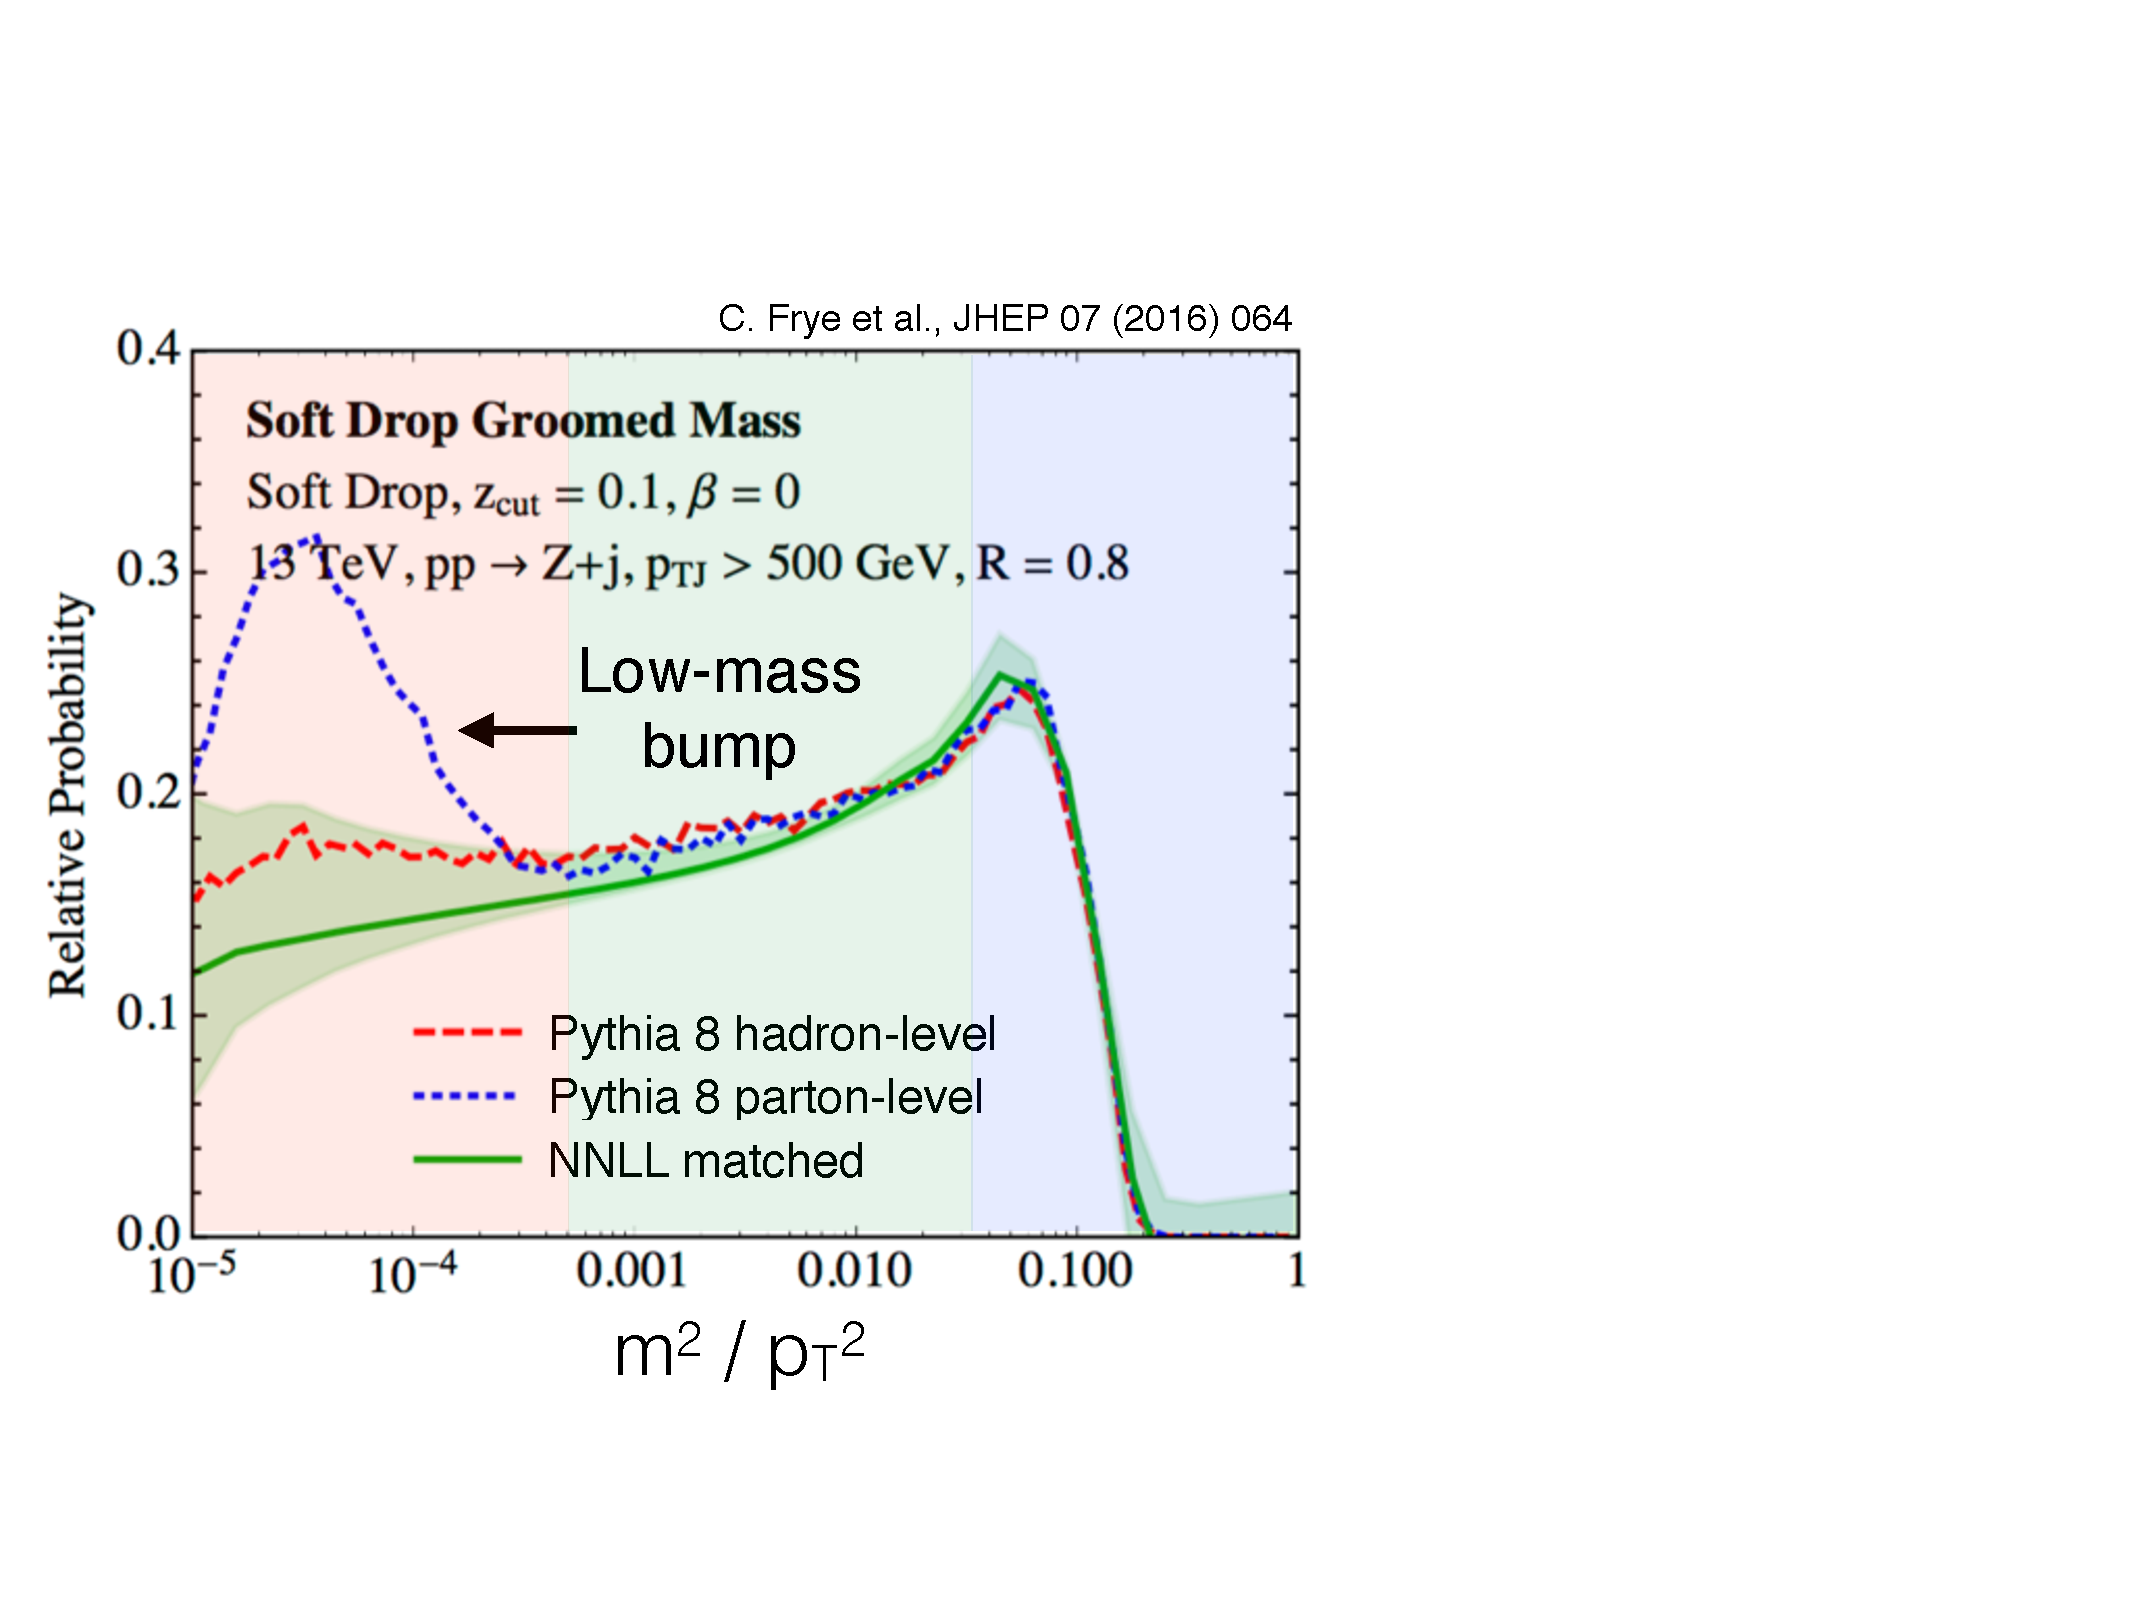
\includegraphics[width=0.5\textwidth]{figs/Lowmassbump.pdf}
\caption{Figure adapted from Ref.~\cite{Frye:2016aiz}.  Replace me with PDF!}
\label{fig:jets:np:illustration}
\end{figure}

\subsection{Monte Carlo tuning with jet substructure observables}
\label{sec:jets:mc}
(Simone, Jennifer, Matt)

Rivet~\cite{Buckley:2010ar}, Professor~\cite{Buckley:2009bj}, HepData~\cite{Buckley:2010jn,Maguire:2017ypu}.  Table with routines (and new ones from this workshop).  See \href{https://twiki.cern.ch/twiki/bin/view/LHCPhysics/LHCJetSubstructureMeasurements}{this twiki}.

\subsubsection{Jet pull}
\label{sec:jets:pull}
(Helen, Vincent, Peter R)

Jet pull~\cite{Gallicchio:2010sw} and measurements~\cite{Aad:2015lxa,Aaboud:2018ibj}.

\subsection{Probing higher-order effects in PSMC}
\label{sec:jets:psmc}

\subsubsection{Bottom up: Triple Collinear Splitting Functions}
(Ben, Eric, Stefan Prestel)

Explain triple collinear functions.  Reference Fig.~\ref{fig:jets:np:triplecollineardiagrams}.

Dire~\cite{Hoche:2015sya}.  PFN~\cite{Komiske:2018cqr}.

\begin{figure}[h!]
\centering
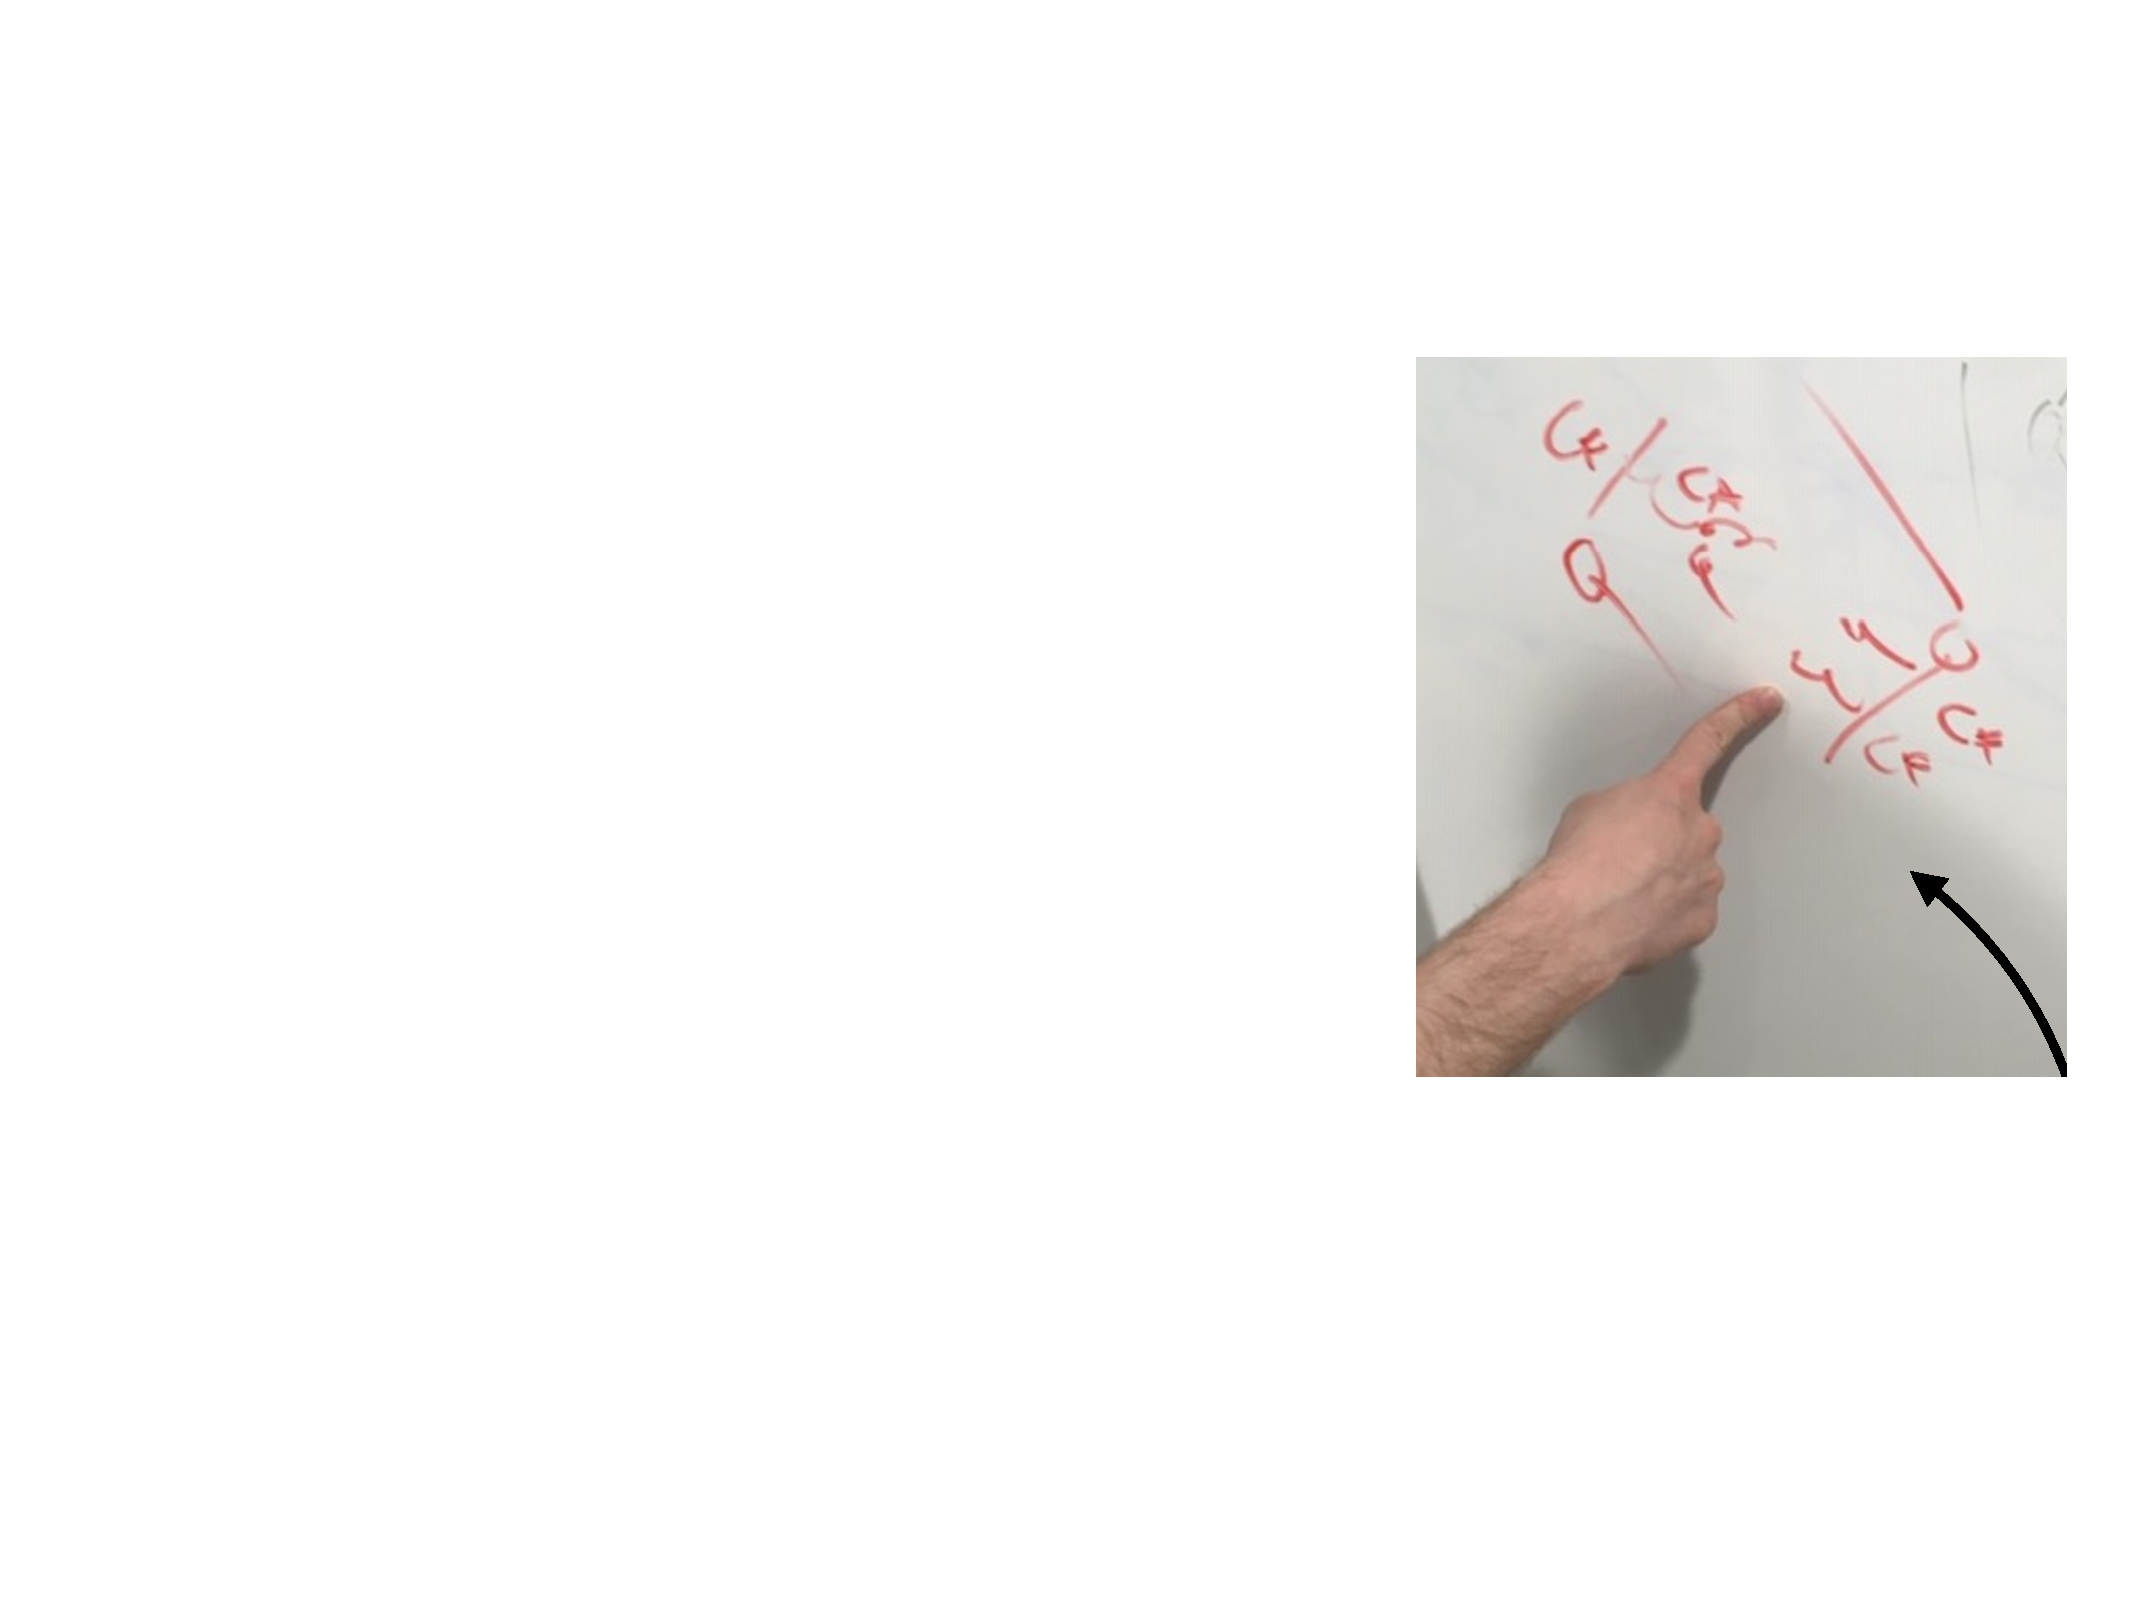
\includegraphics[width=0.45\textwidth]{figs/stefanfinger.pdf}
\caption{Replace me with proper diagrams!}
\label{fig:jets:np:triplecollineardiagrams}
\end{figure}

\begin{figure}[h!]
\centering
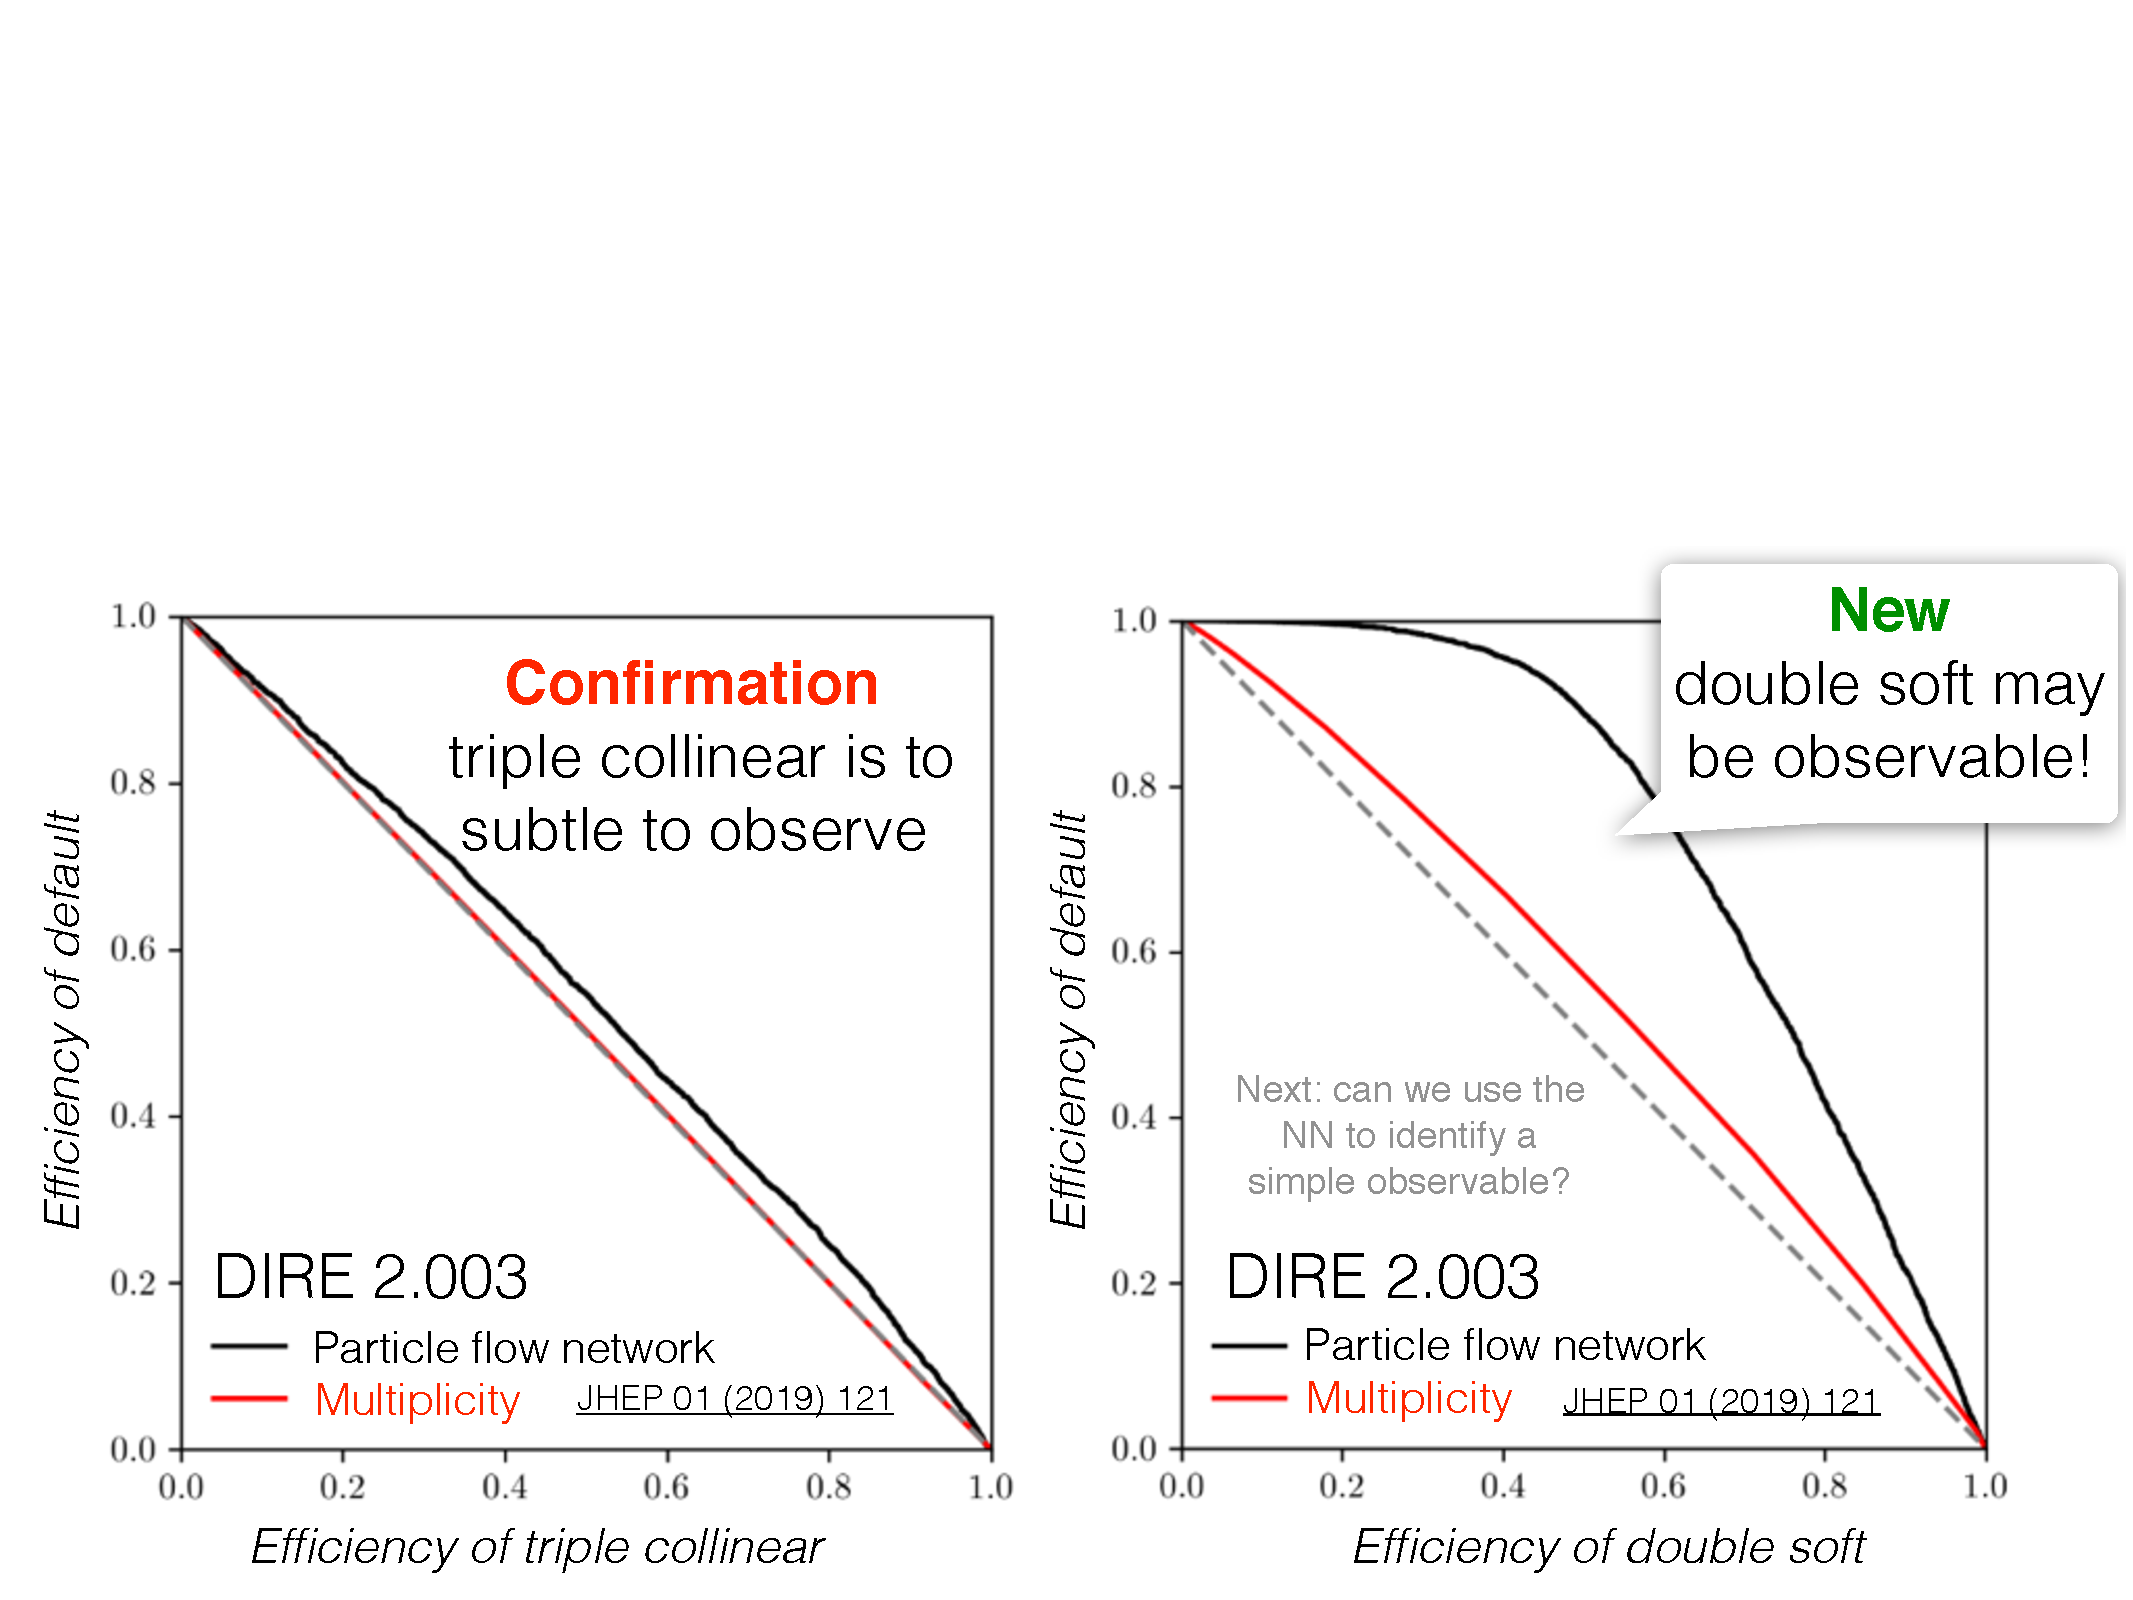
\includegraphics[width=0.85\textwidth]{figs/triplecollinear.pdf}
\caption{Replace me with proper plots!}
\label{fig:jets:np:triplecollinearNN}
\end{figure}


\subsubsection{Top down: $g\to b \bar b$}
\label{sec:jets:gbb}
(Helen, Davide)

\subsection{q/g tagging in VBF and VBS}
\label{sec:jets:vbsbvf}
(Ben, Yachine, Kenneth, Paolo)



\subsection{The gluon PDF (a.k.a Suppressing the QUark in the Region of RElative Large-$x$)}
\label{sec:jets:pdf}

\subsection{The gluon PDF (a.k.a Suppressing the QUark in the Region of RElative Large-$x$)}
(Simone, Gregory, Eric)

Parton Distribution Functions (PDFs) describe the non-perturbative dynamics of quarks and gluons in the protons that take part in high-energy collisions. Therefore, they are a key ingredient for every theoretical prediction that aims to describe particle interactions at high-energy colliders such as the LHC. As a consequence, their precise determination is of utmost importance for LHC phenomenology. 
%
The non-perturbative nature of PDFs hampers their determination from first principles.
%
However, for inclusive enough processes, they are universal, i.e.\, up to power corrections, they do not depend on the particular process, and they can be determined by fitting data from previous experiments. Moreover, although they are themselves non-perturbative objects, their dependence on the energy is governed by the DGLAP equation and the evolution kernels can be computed as a power expansion in the strong coupling. This implies that data collected at past experiments, at different energies, can be used to constrain PDFs. 

Traditionally, the main source of uncertainties assigned to the determination of PDFs arises from the experimental error of the data that enter the fit.~\footnote{Very recently, the inclusion of theory uncertainties in PDF determination has also been achieved~\cite{Harland-Lang:2018bxd,AbdulKhalek:2019ihb,AbdulKhalek:2019bux}} In extreme regions of phase-space, for instance at small- or large-$x$, the experimental uncertainties typically deteriorate and one has to face a reduced number of data points. This is reflected in PDFs which are largely unconstrained in these regions. 
%
For instance, the large PDF uncertainty in the $x\to 1$ region has a negative impact on searches for new and heavy states.
%
 Although this will probably not wash out a potential discovery, it will definitely obscure the nature and the properties of the new state, such as its mass and its couplings. 
%
The way to reduce this PDF uncertainty is to include in the fit data at larger $x$. This cause interesting theoretical issues, because fixed-order perturbation theory becomes less reliable and one should supplement theoretical predictions with threshold resummation, as studied for instance in~\cite{Corcella:2005us,Sato:2013wea,Westmark:2013vea,Bonvini:2015ira,Accardi:2014qda}.


In this study, we focus on the gluon PDF in the region of relatively large longitudinal momentum fraction, $x\sim 10^{-1}$ \sm{check}. The datasets that mostly constrain the gluon in this region are the inclusive jet spectra, in the region of the jet transverse momentum above 1~TeV and the production of top quark pairs. From a theoretical point of view, both processes are known to very high accuracy, i.e. next-to-next-to-leading order (NNLO)~\cite{}. Phenomenologically, the two processes have pros and cons. Inclusive jet production features high statistics across a wide kinematical range and, consequently, even in the high $p_t$ region we are interested the experimental uncertainties do not exceed 10\%. However, because we are measuring inclusive jets we cannot distinguish the flavour content and the cross section is dominated by quark-quark scattering, which bear little information about the gluon PDF. 
%
On the other hand, at LHC energies, top pair production is dominated by gluon fusion and therefore offers a direct probe of the gluon luminosity. In this case, however, we pay a much higher price in terms of experimental uncertainties, essentially because we run out of statistics of values of the top transverse momentum much smaller than for inclusive jets. 
%
Ideally, we would like to exploit the vast jet samples collected by the LHC experiments to tease out more information about the gluon PDF. We immediately realise that one way of achieving this scope would be to supplement the inclusive jet $p_t$ spectrum with some information about the jet flavour. That is, we are going to explore the possibility of using the \emph{inclusive gluon-jet $p_t$} spectrum to extract parton densities, rather than its flavour-blind version.  Properly defining quark jets versus gluon jets is a very active area of jet substructure~\cite{} and indeed it was one of the focus of a past edition of the Les Houches proceedings~\cite{Badger:2016bpw} (see also the follow-up study~\cite{Gras:2017jty}). 


\begin{figure}
\begin{center}
\includegraphics[width=0.49\textwidth, page=9]{figs/fractions.pdf} \hfill
\includegraphics[width=0.49\textwidth, page=10]{figs/fractions.pdf}
\caption{Born-level studies of the flavour composition of dijet events at $\sqrt{s}=13$~TeV, as a function of the jet transverse momentum. The plot on the left shows the fractions of quark-initiated and gluon-initiated processes that contribute to a $gg$ final state. The plot of the right instead shows the fractional composition of the final state for any initial state.}
\label{fig:born_studies} 
\end{center}
\end{figure}

Before discussing how we can sensibly attach a flavour tag to a jet, let us perform a zeroth order test of this idea. Let us assume that we can indeed tag a gluon jet in the final state, the obvious question we should ask ourselves is how strongly the flavour of the final state, which we measure, is correlated with the flavour of the initial state, which intimately related to the parton densities we want to study. 
%
We can easily assess this correlation at Born level by explicitly consider $2 \to 2$ parton scattering and focussing on the two gluon ($gg$) final state. The left-hand plot of Fig.~\ref{fig:born_studies} shows the fraction of the $gg$ final state that originates from quark-anti-quark initial state ($q \bar q \to gg$) in red and the one from gluon-gluon initial state ($gg \to gg$)  in blue, as a function of the final-state transverse momentum for proton-proton collisions at $\sqrt{s}=13$~TeV (the plot uses the NLO PDF set CT14~\cite{Dulat:2015mca}). 
%
The result of this very first study is rather encouraging: in the region $p_t=1,2$~TeV we are interested, there is indeed very strong correlation between the initial- and final-state flavours. This is, of course, only a Born-level study and we can reasonably expect this correlation to deteriorate at higher-orders mostly due to large-angle radiation. 
%
Although a quantitative estimate of these effects goes beyond the scope of these proceedings, we do not expect them to be dramatic. In any case, one could in principle reduce such contributions with jet grooming. 
%
With the same Born-level setup, we can study how the different partonic final states contribute to the inclusive cross section. This is shown on the right-hand plot of Fig.~\ref{fig:born_studies}. As $p_t$ increases, the fraction of final-state quark rapidly increases. Indeed, the region of interest the $gg$ final state represents less than 10\% of the inclusive sample. This makes the enterprise of enhancing the $gg$ contributions (or, equivalently, suppressing the quarks) particularly challenging. 



\begin{figure}
\begin{center}
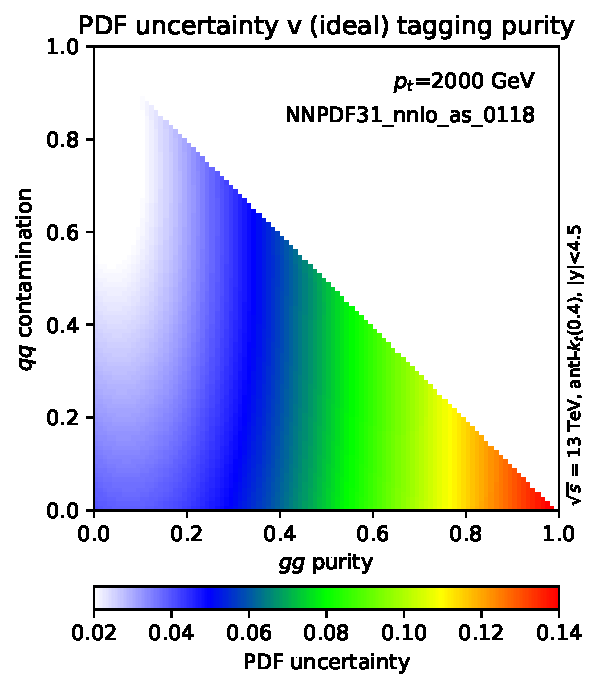
\includegraphics[width=0.42\textwidth, page=1]{figs/performance-plots.pdf} \hfill
\includegraphics[width=0.49\textwidth, page=2]{figs/performance-plots.pdf}
\caption{}
\label{fig:pdf_unc_studies} 
\end{center}
\end{figure}

The next step in our study is to evaluate the current PDF uncertainties, as a function of the final-state flavour composition. 
%
In order to do so, we imagine as a fist step to have at our disposal an idealised tagging procedure that allows us to freely enhance or depress the different partonic components of the final state. We will come back to actual realisations of this tagger later. 
%
In this context, we find useful to define the gluon-gluon ($gg$) purity as
\begin{equation}
gg \, \text{purity}= \frac{\sigma_{gg}}{\sigma_{qq}+\sigma_{qg}+\sigma_{gg}},
\end{equation}
where $\sigma_{ij}$ is the cross section for producing parton $i$ and $j$, evaluated at Born level.  In an analogous way, we can also define the $q q$ contamination is defined analogously, while $q g$ is then fixed by unitarity. Then, for given values $gg$ purity and $qq$ contamination we can evaluate the PDF uncertainty on the cross section.
%
 We decide to perform this estimate using the NNLO PDF set from NNPDF3.1~\cite{Ball:2017nwa} for jets at $2$~TeV.
 %
%The results are shown in Fig.~\ref{fig:pdf_unc_studies}, on the left. 
%
We actually already know from Fig.~\ref{fig:born_studies}, that in the inclusive, i.e.\ untagged, case correspond to $gg$ purity of the order 5\% at $p_t=2$~TeV, while $qq$ and $qg$ makes up roughly 55\% and 40\% of the inclusive sample, respectively. 
%
From the left-hand plot on Fig.~\ref{fig:pdf_unc_studies}, we can then read-off the PDF uncertainty to be of the order of a few percent. This is reflects the fact that the quark parton densities are fairly-well constrained in the region of interest. 
As we move to higher values of the $gg$ purity, the less constrained gluon PDFs start to play a more significant role and, as a consequence, the overall uncertainties goes up. For instance, if we were able to devise a tagger that purifies the $gg$ final state to 80\%, we would increase the PDF uncertainty from 2\% to 12\%. 


\begin{figure}
\begin{center}
\includegraphics[width=0.49\textwidth, page=4]{figs/performance-plots.pdf} \hfill
\includegraphics[width=0.49\textwidth, page=5]{figs/performance-plots.pdf}
\caption{}
\label{fig:performance_studies} 
\end{center}
\end{figure}


\subsubsection{The highest energy gluons at the LHC}
\label{sec:jets:highest}
(Ben)

\subsection{Conclusion and Outlook}
\label{sec:jets:conclusion}
(Simone)

\subsection*{Acknowledgments}

We thank the participants of Les Houches 2019 for a lively environment and useful discussions.
%%
BN is supported in part by the Office of High Energy Physics of the U.S. Department of Energy under Contract No. DE-AC02-05CH11231.
%
SM is also supported by the curiosity-driven grant "Using jets to challenge the Standard Model of particle physics" from Universit\`a di Genova.

\bibliography{lh2019}

\end{document}
